\ChapterImageStar[cap:dar]{Análisis de Decisiones y Resolución}{./images/fondo.png}\label{cap:dar}
\mbox{}\\

\section{Metodología de evaluación}

La metodología de evaluación aplicada para la selección de las tecnologías correspondientes a los Sistemas de Detección y Prevención de 
Intrusiones (\IDPS) y a la Gestión de Eventos e Información de Seguridad (\SIEM) fue \DAR\ (\textit{Decision Analysis and Resolution}) de 
\CMMI~\cite{CMMIInstitute2010}. Esta metodología permitió evaluar las necesidades del grupo \GRID\ mediante un proceso estructurado en el 
que se consideraron múltiples alternativas, criterios de evaluación definidos y un análisis comparativo basado en controles relacionados 
con las normas ISO/IEC 27001 e ISO/IEC 27017, alineados con el panorama actual y los objetivos del grupo.

En este contexto, se identificaron y analizaron diversas tecnologías \IDPS y \SIEM, aplicando criterios como rentabilidad, tipo de licencia, 
documentación, soporte y compatibilidad, utilizando como fuentes de información sus respectivas documentaciones oficiales y repositorios en 
GitHub. De esta manera, el uso de \DAR\ aportó transparencia, trazabilidad y justificación técnica al proceso de selección de las tecnologías 
orientadas al fortalecimiento de la seguridad de la infraestructura del grupo de investigación \GRID.

\subsection{Lista de criterios}

En esta sección se presenta la descripción de los criterios de evaluación utilizados en las tablas comparativas de tecnologías. Cabe 
resaltar que, con apoyo de las normas \ISO/IEC 27001 e \ISO/IEC 27017, fue posible definir la mayoría de los criterios empleados para 
determinar la pertinencia y capacidad de cada herramienta frente a los requerimientos de seguridad establecidos para la infraestructura del 
grupo \GRID.

\subsection{Criterios generales}

Los criterios expuestos a continuación corresponden a los utilizados en ambas tablas del análisis \DAR y permiten evaluar, de manera 
integral, las características que debe cumplir una herramienta para que su implementación se ajuste a las necesidades, problemáticas y 
oportunidades de la organización. Parte de estos criterios fueron adaptados del estudio realizado por~\cite{hadi2024opensource}, en el 
cual se desarrolla una evaluación similar de herramientas con fines de selección y adopción tecnológica.

\subsubsection{Rentabilidad}

Este criterio se fundamentó en el estudio de~\cite{hadi2024opensource} y permite evaluar la relación entre el beneficio esperado de la 
herramienta y los costos asociados a su adopción y mantenimiento. Asimismo, considera si la solución ofrece un valor adecuado frente a la 
inversión requerida, incluyendo aspectos relacionados con infraestructura, soporte y operación.

\subsubsection{Tipo de licencia}

Este criterio analiza el modelo de licenciamiento de la herramienta, considerando si corresponde a una solución de código abierto, 
comercial o híbrida. Asimismo, permite valorar aspectos relacionados con la flexibilidad de uso, restricciones legales, costos de 
adquisición y posibilidades de personalización.

\subsubsection{Documentación}

Este criterio se fundamenta en el control A.5.37 de la \ISO/IEC 27001~\cite{iso27001} y permite evaluar la disponibilidad, calidad, 
actualización y nivel de detalle de la documentación técnica y funcional de la herramienta. Entre la documentación considerada se incluyen 
manuales de instalación, configuración y administración, así como casos de uso y guías para la solución de problemas.

\subsubsection{Facilidad de uso}

Este criterio se fundamentó en el estudio de~\cite{hadi2024opensource} y permite evaluar el nivel de complejidad que presenta la 
herramienta para su instalación, configuración, operación y administración. Asimismo, considera aspectos como la curva de aprendizaje, la 
usabilidad de la interfaz y la facilidad de adopción por parte del equipo técnico.

\subsubsection{Escalabilidad}

Este criterio se fundamenta en el estudio de~\cite{hadi2024opensource} y permite evaluar la capacidad de la herramienta para adaptarse al 
crecimiento de la infraestructura, soportando un mayor volumen de datos, eventos, usuarios o nodos sin degradar significativamente su 
rendimiento.

\subsubsection{Consumo de recursos}

Este criterio analiza la cantidad de recursos computacionales requeridos por la herramienta, incluyendo CPU, memoria, almacenamiento y 
ancho de banda. Asimismo, resulta fundamental para evaluar su viabilidad operativa dentro de la infraestructura cloud objetivo.

\subsubsection{Popularidad}

Valora el nivel de adopción y reconocimiento de la herramienta dentro de la comunidad técnica y científica. Este criterio usa como medida 
la suma de las descargas y forks de la respectiva página GitHub.

\subsection{Criterios de Tecnologías IDPS}

\subsubsection{Precisión de detección}

Este criterio se encuentra alineado con el control A.5.7 de la \ISO/IEC 27001~\cite{iso27001} y permite evaluar la capacidad de la 
herramienta para identificar correctamente eventos maliciosos, anomalías o patrones de ataque dentro del tráfico de red, minimizando 
omisiones en la detección de amenazas reales.

\subsubsection{Tasa de falsos positivos}

Este criterio se encuentra alineado con el control A.5.24 de la \ISO/IEC 27001~\cite{iso27001} y permite medir la frecuencia con la que la 
herramienta genera alertas incorrectas frente a tráfico legítimo. Un valor alto en este criterio indica una mayor confiabilidad operativa y 
una menor carga para el personal encargado del monitoreo del tráfico.

\subsubsection{Integración con otros sistemas}

Este criterio determina la facilidad con la que la herramienta puede interoperar con otras soluciones de seguridad, monitoreo, SIEM, 
\textit{firewalls}, plataformas cloud y sistemas de gestión institucional.

\subsubsection{Capacidad de detección por comportamiento}

Este criterio se estructura conforme al control A.8.16 de la \ISO/IEC 27001~\cite{iso27001} y permite evaluar la capacidad del IDPS para 
identificar amenazas a partir de comportamientos anómalos o patrones no basados exclusivamente en firmas, facilitando la detección de 
ataques desconocidos o variantes avanzadas.

\subsubsection{Actualización de firmas}

Este criterio se deriva del control A.5.7 de la \ISO/IEC 27001~\cite{iso27001} y permite analizar la disponibilidad, frecuencia y facilidad 
de actualización de las reglas, firmas o bases de conocimiento utilizadas para detectar amenazas conocidas. Asimismo, este criterio 
resulta fundamental para responder oportunamente a nuevas vulnerabilidades y vectores de ataque.

\subsection{Criterios de Tecnologías SIEM}
\subsubsection{Capacidad de correlación de eventos}

Este criterio se encuentra alineado con el control CLD 12.4.5 de la \ISO/IEC 27017~\cite{iso27017} y permite evaluar la capacidad de la 
herramienta para correlacionar múltiples eventos provenientes de diferentes fuentes, con el fin de identificar patrones de ataque, 
incidentes complejos o comportamientos anómalos que no serían evidentes al analizar los eventos de manera aislada.

\subsubsection{Volumen de eventos por segundo (EPS)}

Este criterio se encuentra alineado con el control CLD 12.4.5 de la \ISO/IEC 27017~\cite{iso27017} y permite evaluar la capacidad de la 
herramienta para correlacionar múltiples eventos provenientes de diferentes fuentes, con el fin de identificar patrones de ataque, 
incidentes complejos o comportamientos anómalos que no serían evidentes al analizar los eventos de manera aislada.

\subsubsection{Calidad de alertas generadas}

Este criterio se establece a partir del control CLD.12.4.5 de la \ISO/IEC 27017~\cite{iso27017} y permite analizar la precisión, relevancia 
y nivel de detalle de las alertas emitidas por la herramienta. Asimismo, considera la capacidad de priorizar incidentes críticos, reducir 
el ruido operativo y proporcionar contexto suficiente para la toma de decisiones.

\subsubsection{Cumplimiento normativo}

Este criterio se estructura conforme al control A.5.31 de la norma \ISO/IEC 27001~\cite{iso27017}, con el propósito de determinar el 
grado en que la herramienta facilita el alineamiento con estándares, marcos regulatorios y buenas prácticas de seguridad, tales como 
\ISO/IEC 27001, \ISO/IEC 27017 e \ISO/IEC 27018. Asimismo, incluye capacidades de soporte para la trazabilidad, auditoría y generación de 
evidencias.

\subsubsection{Dashboards e informes}

Este criterio se construyó conforme a lo establecido en el control 12.4.1 de la norma \ISO/IEC 27017~\cite{iso27017}, con el fin de evaluar la 
calidad visual y funcional de los paneles de monitoreo, así como la capacidad de la herramienta para generar informes automáticos, 
personalizados y orientados a auditoría, operación o gestión ejecutiva.

\subsection{Lista de Tecnologías}
Tras definir los criterios, se identificaron las siguientes tecnologías \IDPS:
\begin{itemize}
	\item Snort
	\item OSSEC
	\item Zeek
	\item Suricata
\end{itemize}

Tras definir los criterios, se identificaron las siguientes tecnologías \SIEM:
\begin{itemize}
	\item OSSIM
	\item ELK Stack
	\item Graylog
	\item Wazuh
	\item Apache Metron
\end{itemize}

\subsection{Análisis DAR}

Con los criterios definidos y las tecnologías identificadas, se procede a realizar el análisis \DAR. Para este análisis se utilizó 
una metodología estructurada basada las plantillas encontradas en el Apéndice~\ref{chap:plantilla-dar}. que permite evaluar 
sistemáticamente cada tecnología IDPS y SIEM contra los criterios establecidos.

Los resultados del análisis \DAR de las tecnologías \IDPS se presentan en la Figura~\ref{fig:resultados-idps} y los resultados de las 
tecnologías \SIEM en la Figura~\ref{fig:resultados-siem}, donde cada tecnología fue evaluada con un rango de valoración de 1 a 5, en el 
cual el valor de 1 significa que no cumple en absoluto con el criterio evaluado y 5 que cumple de manera satisfactoria con el mismo.

\begin{figure}[H]
	\centering
	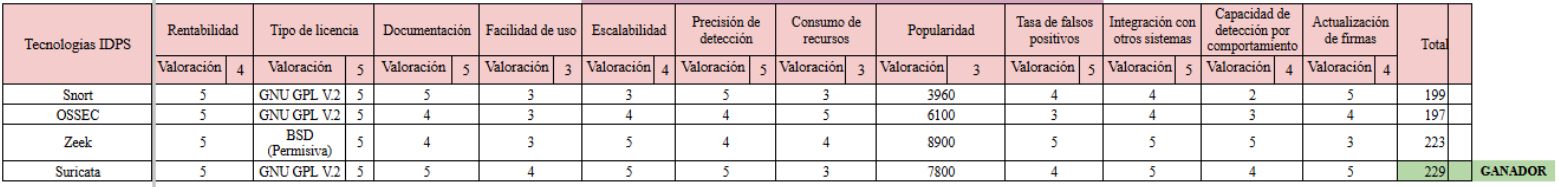
\includegraphics[scale=0.4] {tablas-images/dar/resultados-idps.png}
	\caption{Resultados del análisis DAR para tecnologías IDPS}\label{fig:resultados-idps}
\end{figure}

\begin{figure}[H]
	\centering
	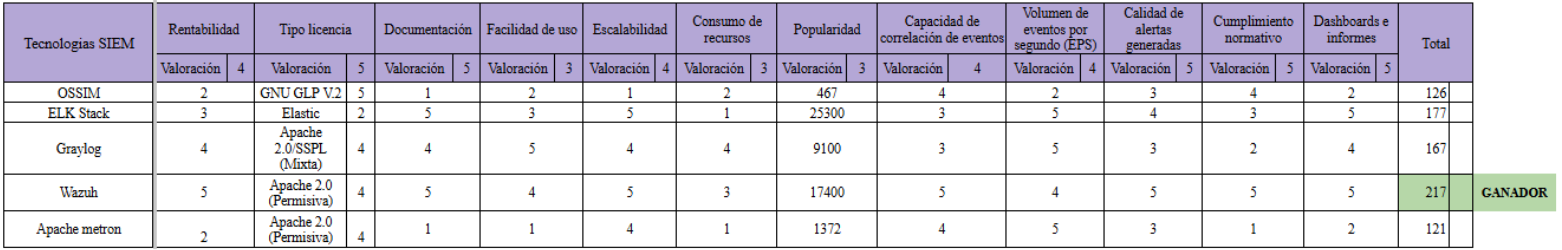
\includegraphics[scale=0.4] {tablas-images/dar/resultados-siem.png}
	\caption{Resultados del análisis DAR para tecnologías SIEM}\label{fig:resultados-siem}
\end{figure}

\section{Resultados}

\subsection{Resumen del análisis}

En este apartado se presentan las tecnologías seleccionadas en cada análisis DAR realizado, de acuerdo con el valor más alto obtenido en 
la sumatoria calculada a partir de los criterios propuestos y su pertinencia dentro del contexto del estudio.

\subsection{Suricata}

La herramienta Suricata se posiciona como la tecnología ganadora dentro de la categoría IDPS, debido a los resultados obtenidos en cada 
uno de los criterios evaluados. La herramienta alcanzó una valoración total de 229 puntos, evidenciando un rendimiento superior frente a 
las demás alternativas analizadas.

No obstante, Zeek también presentó resultados relevantes dentro del análisis, obteniendo un total de 223 puntos, posicionándose como la 
segunda tecnología con mejor valoración. Aunque las demás herramientas evaluadas cumplen con funcionalidades relacionadas con la detección 
y prevención de intrusiones, estas no se ajustan completamente a las necesidades, problemáticas y oportunidades actuales del grupo de 
investigación \GRID.

En la Figura~\ref{fig:estadistica-idps} se presentan las puntuaciones obtenidas por cada herramienta IDPS durante el análisis realizado.

\begin{figure}[H]
	\centering
	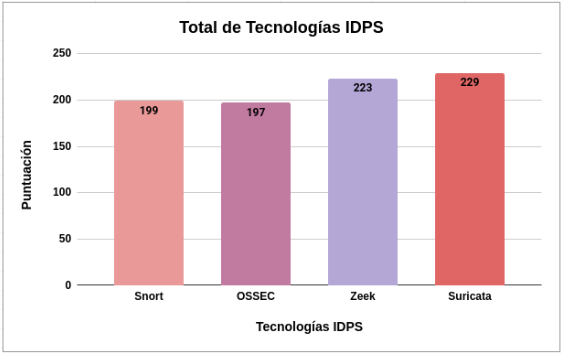
\includegraphics[scale=0.5] {tablas-images/dar/estadistica-idps.png}
	\caption{Gráfico del análisis DAR para tecnologías IDPS}\label{fig:estadistica-idps}
\end{figure}

\subsection{Wazuh}

La herramienta Wazuh se posiciona como la tecnología seleccionada dentro de la categoría SIEM, debido a los resultados obtenidos en los criterios establecidos para su evaluación. La herramienta alcanzó una valoración total de 217 puntos, reflejando un desempeño superior frente a las demás alternativas analizadas.

Por otra parte, ELK Stack obtuvo una valoración de 177 puntos, posicionándose como una alternativa viable dentro del análisis. Sin embargo, sus características no se alinean completamente con las necesidades y requerimientos identificados en el análisis de necesidades, problemáticas y oportunidades (NPO) del grupo de investigación \GRID.

En la Figura~\ref{fig:estadistica-siem} se presentan las puntuaciones obtenidas por cada herramienta SIEM evaluada en el análisis DAR.

\begin{figure}[H]
	\centering
	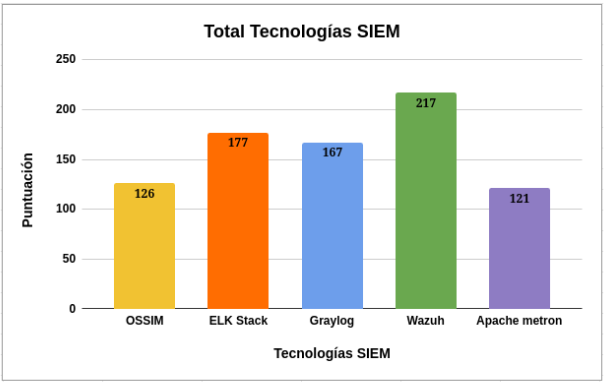
\includegraphics[scale=0.5] {tablas-images/dar/estadistica-siem.png}
	\caption{Gráfico del análisis DAR para tecnologías SIEM}\label{fig:estadistica-siem}
\end{figure}

\subsection{Próximos pasos}
Se procede con el diseño de las arquitecturas de la solución con cada universo y su posterior implementación a través de un prototipo 
funcional.
